\documentclass[slidestop, compress, mathserif, containsverbatim, xcolor=dvipsnames]{beamer}

%tema
\usetheme{Antibes}
\usecolortheme[named=Maroon]{structure}
\usecolortheme{beaver}

%dno slajdova
\setbeamertemplate{footline}[frame number]
\usenavigationsymbolstemplate{}

%izgled blokova
\useinnertheme[shadow=true]{rounded}
%\setbeamercolor{block title}{use=structure,fg=white,bg=brown3!75!black}
%\setbeamercolor{block body}{use=structure,fg=black,bg=lightgray!20!white}


%outline za svaki odeljak
\AtBeginSection[]
{
  \begin{frame}[squeeze]{}
    \tableofcontents[currentsection]
  \end{frame}
}



\usepackage{graphicx}
\usepackage{pgf}
\usepackage{wrapfig}
\usepackage{amsmath}
\usepackage{amssymb}
\usepackage{gclc}

\usepackage[serbian]{babel}
\usepackage[utf8]{inputenc}
\usepackage[T2A]{fontenc}

\usepackage{amssymb}
\usepackage{gclc}
\usepackage{stmaryrd}
\usepackage{tikz}


\newcommand{\agbett}[3]{\ensuremath{\mathcal{B}_T^{\mathit{ag}}\ #1\ #2\ #3}}
\newcommand{\agbeth}[3]{\ensuremath{\mathcal{B}_H^{\mathit{ag}}\ #1\ #2\ #3}}
\newcommand{\agcongr}[4]{\ensuremath{#1#2 \cong^{ag} #3#4}}
\newcommand{\aginh}[2]{\ensuremath{#1 \in^{ag}_H #2}}
\newcommand{\agtransp}[2]{\ensuremath{transp^{ag}\ #1\ #2}}
\newcommand{\agtransl}[2]{\ensuremath{trans^{ag}_l\ #1\ #2}}
\newcommand{\agrotp}[2]{\ensuremath{rotp^{ag}\ #1\ #2}}
\newcommand{\agsymp}[1]{\ensuremath{symp^{ag}\ #1}}
\newcommand{\agrotl}[2]{\ensuremath{rotl^{ag}\ #1\ #2}}
\newcommand{\agsqdist}[2]{\ensuremath{d^2_{ag}\ #1\ #2}}
\newcommand{\ag}[2]{\ensuremath{^{ag}\ #1\ #2}}


\newcommand{\bett}[3]{\ensuremath{\mathcal{B}_t(#1, #2, #3)}}
\newcommand{\colint}[3]{\ensuremath{\mathcal{C}_t(#1, #2, #3)}}
\newcommand{\congrt}[4]{\ensuremath{#1#2 \cong_t #3#4}}

\newcommand{\inh}[2]{\ensuremath{#1 \in_h #2}}
\renewcommand{\beth}[3]{\ensuremath{\mathcal{B}_h(#1, #2, #3)}}
\newcommand{\colinh}[3]{\ensuremath{\mathcal{C}_h(#1, #2, #3)}}
\newcommand{\congrh}[4]{\ensuremath{#1#2 \cong_h #3#4}}

\newcommand{\vect}[1]{\vec{#1}}


\usepackage{amsmath}
\usepackage{amssymb}
\usepackage{stmaryrd}
\usepackage{url}
\usepackage{graphicx}
\usepackage{wasysym}
\usepackage{mathtools}

\newcommand{\lbrakk}{\llbracket}
\newcommand{\rbrakk}{\rrbracket}
\newcommand{\cnj}[1]{\overline{#1}}
\renewcommand{\C}[0]{\ensuremath{\mathbb{C}}}
\newcommand{\extC}[0]{\ensuremath{\overline{\C}}}
\newcommand{\Repnzv}[1]{\ensuremath{\lfloor#1\rfloor_{C2}}}
\newcommand{\Absnzv}[1]{\ensuremath{\lceil#1\rceil^{C2}}}
\newcommand{\stpr}[1]{sp\ #1}
\newcommand{\Reprs}[1]{\ensuremath{\lfloor#1\rfloor_{R3}}}
\newcommand{\Absrs}[1]{\ensuremath{\lceil#1\rceil^{R3}}}
\newcommand{\Reprm}[1]{\ensuremath{\lfloor#1\rfloor_{M}}}
\newcommand{\Absrm}[1]{\ensuremath{\lceil#1\rceil^{M}}}
\newcommand{\Repcm}[1]{\ensuremath{\lfloor#1\rfloor_{H}}}
\newcommand{\Abscm}[1]{\ensuremath{\lceil#1\rceil^{H}}}
\newcommand{\Reppl}[1]{\ensuremath{\lfloor#1\rfloor_{R4}}}
\newcommand{\Abspl}[1]{\ensuremath{\lceil#1\rceil^{R4}}}
\newcommand{\approxhc}{\ensuremath{\approx_{C2}}}
\newcommand{\approxrm}{\ensuremath{\approx_{M}}}
\newcommand{\approxcm}{\ensuremath{\approx_{cm}}}
\newcommand{\approxocm}{\ensuremath{\approx_{ocm}}}
\newcommand{\approxp}{\ensuremath{\approx_{R4}}}
\newcommand{\ofocircline}[1]{{#1}^{\ocircle}}
\newcommand{\ofcircline}[1]{{#1}^{\circlearrowleft}}
\newcommand{\oppocircline}[1]{{#1}^{\leftrightarrow}}

\newcommand{\RepRt}[1]{\ensuremath{\lfloor#1\rfloor_{R3}}}
\newcommand{\AbsRt}[1]{\ensuremath{\lceil#1\rceil^{R3}}}

\def\d{{\fontencoding{T1}\selectfont\dj}}
\def\D{{\fontencoding{T1}\selectfont\DJ}}


%za sirinu tabele
\usepackage{array}
\newcolumntype{L}[1]{>{\raggedright\let\newline\\\arraybackslash\hspace{0pt}}m{#1}}
\newcolumntype{C}[1]{>{\centering\let\newline\\\arraybackslash\hspace{0pt}}m{#1}}
\newcolumntype{R}[1]{>{\raggedleft\let\newline\\\arraybackslash\hspace{0pt}}m{#1}}

\title{Формализација различитих модела геометрије и примене у
  верификацији аутоматских доказивача теорема}

\author[Данијела Симић]{Данијела Симић\\{\small Ментор: др Филип Марић}}
\institute{Математички факултет \\ Универзитет у Београду}
\date{8.08.2017.}

\begin{document}

\begin{frame}
\titlepage
\end{frame}

%Uvod
\section{Увод}

\begin{frame}{Увод}
  \begin{itemize}
  \item Различите геометрије:
     \begin{itemize}
     \item Еуклидска геометрија
     \item Хиперболичка геометрија
     \end{itemize} \vfill
   \item Различити приступи изучавања:
     \begin{itemize}
     \item Синтетички приступ:
       \begin{itemize}
       \item аксиоматски систем Хилберта
       \item аксиоматски систем Тарског
       \end{itemize}
     \item Аналитички приступ:
       \begin{itemize}
       \item у Декартовој координатној равни
       \item у комплексној равни
       \end{itemize}
     \end{itemize}\vfill
  \end{itemize}
\end{frame}

\section{Доказивање у геометрији}
\begin{frame}{Доказивање у геометрији}
  \begin{itemize}
  \item Грешке у математичким доказима. \vfill
  \item Механички провериви докази. \vfill
  \item Интерактивни доказивачи теорема. \vfill
  \item Аутоматски доказивачи теорема. \vfill
  \end{itemize}
\end{frame}

%Interaktivni dokazivaci teorema
\section{Интерактивни доказивачи теорема}

\begin{frame}{Интерактивни доказивачи теорема}
  \begin{itemize}
  \item Карактеристике интерактивних доказивача теорема. \vfill
  \item Важни резултати:
    \begin{itemize}
    \item Основна теорема алгебре
    \item Геделова теорема непотпуности
    \item многе теореме реалне анализе
    \item формални доказ теореме о обојивости графа са 4 боје
    \item формално верификован компилатор за програмски језик $C$
    \item формално верификован оперативни систем
    \item прва група Хилбертових аксиома и последице
    \item велики делови књиге Тарског
    \end{itemize}\vfill
  \end{itemize}
\end{frame}

{
\setbeamertemplate{navigation symbols}{}
\begin{frame}[plain]{Isabelle/HOL}
    \makebox[\linewidth]{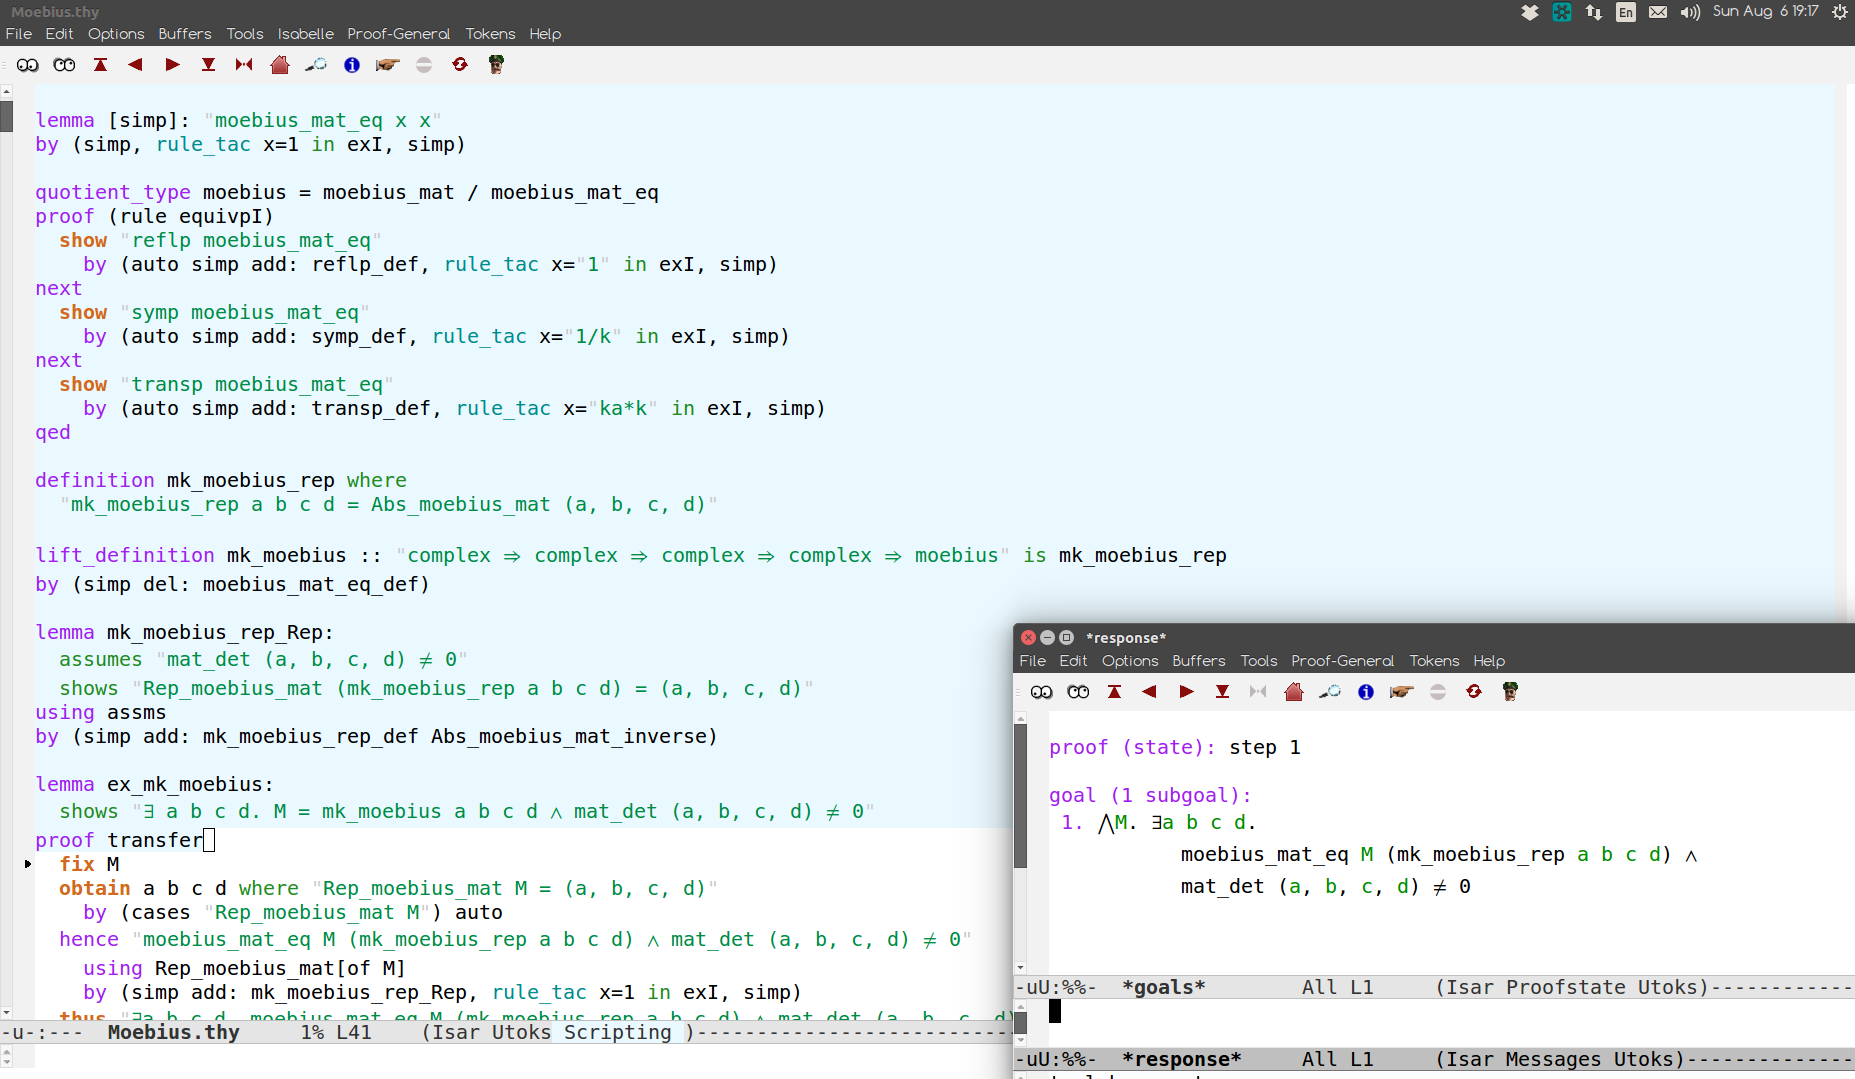
\includegraphics[width=\paperwidth]{./slike/isabelleHOL.png}}
\end{frame}
}


%Dokazivanje u geometriji
\section{Аутоматско доказивање геометријских теорема}

\begin{frame}{Аутоматско доказивање геометријских теорема}
  \begin{itemize}
  \item Алгебарски доказивачи -- Вуов метод и метод Гребнерових база. \vfill
  \item Синтетички доказивачи. \vfill
   \item Полусинтетички доказивачи --  метод површина, метод пуног угла, метод запремине.\vfill
  \item Везе између интерактивних и аутоматских доказивача. \vfill
  \end{itemize}
\end{frame}

\section{Мотивација и циљеви}

\begin{frame}{Мотивација и циљеви}
  \begin{itemize}
  \item Верификација аутоматских доказивача теорема. \vfill
  \item Формализација мета--теорије потребне да се искаже и докаже
    коректност алгебарских метода. \vfill
  \item Развој и прилагођавање алгебарских метода.
  \end{itemize}
\end{frame}

%Formalizacija analiticke geometrije
\section{Формализација геометрије Декартове равни}

\begin{frame}{Циљеви формализације геометрије Декартове равни}
  \begin{itemize}
  \item Формализација Декартове координатне равни. \vfill
  \item Различите дефиниције су еквивалентне. \vfill
  \item Стандардна геометрија координатне равни представља модел
    аксиоматског система Тарског. \vfill
  \item Декартова координатна раван задовољава већину аксиома Хилберта. \vfill
  \item Упоредити ове две формализације. \vfill
  \end{itemize}
\end{frame}

\begin{frame}[shrink, squeeze]{Основни појмови}
  \begin{itemize}
  \item Тачке: {\tt {\bf type\_synonym}\ point$^{ag}\ =\ $"$real \times real$"\ }
  \item Распоред тачака: $\mathcal{B}(A, B, C)$
    \begin{block}{Релација \emph{између} у геометрији Тарског}
      {\tt
        \begin{tabbing}
          \hspace{5mm}\=\hspace{5mm}\=\kill
          {\bf definition} "$\agbett{(xa, ya)}{(xb, yb)}{(xc, yc)} \longleftrightarrow$\\
      \>$(\exists (k::real).\ 0 \le k \ \wedge\ k \le 1 \ \wedge$\\
      \>\>$(xb - xa) = k \cdot (xc - xa) \ \wedge\ (yb - ya) = k \cdot (yc - ya))$"
        \end{tabbing}
      }
    \end{block}
  \item Релација подударно: $\congrt{A}{B}{C}{D}$
    \begin{block}{Релација подударно}
      {\tt
        \begin{tabbing}
          {\bf definition} "$\agsqdist{(x_1, y_1)}{(x_2, y_2)} =$ \= $(x_2-x_1)\cdot (x_2-x_1)+$ \\
           \> $(y_2-y_1)\cdot (y_2-y_1)$"\\
          {\bf definition} "$\agcongr{A_1}{B_1}{A_2}{B_2} \longleftrightarrow \agsqdist{A_1}{B_1} = \agsqdist{A_2}{B_2}$"
        \end{tabbing}
      }
    \end{block}
  \end{itemize}
\end{frame}

\begin{frame}{Правa}
  \begin{itemize}
  \item $Ax + By + C = 0$ ($kAx + kBy + kC = 0$, $k \neq 0$) \vfill
  \item \begin{tabbing}
        {\bf typedef} line\_coeffs$^{ag}$ $=$ \\
        \hspace{5mm}"$\{((A::real), (B::real), (C::real)).\ A \neq 0 \vee B \neq 0\}$"
  \end{tabbing} \vfill
  \item {\tt
    \begin{tabbing}
      \hspace{5mm}\=\kill
      {\bf definition} "$l_1 \approx^{ag} l_2$ $\longleftrightarrow$ \\
      \>  $(\exists\ A_1\,B_1\,C_1\,A_2\,B_2\,C_2.$\\
      \>  $\RepRt{l_1} = (A_1, B_1, C_1)) \ \wedge\ \RepRt{l_2} = (A_2, B_2, C_2)\ \wedge$\\
      \>  $(\exists k.\ k \neq 0 \,\wedge\, A_2 = k\cdot A_1 \,\wedge\,  B_2 = k\cdot B_1\,\wedge\,C_2 = k\cdot C_1))$"
    \end{tabbing}
  }
    
  \begin{block}{}
    Права (тип {\tt line$^{ag}$}) се дефинише коришћењем {\tt
    quotient\_type} команде као \structure{класа еквиваленције над
    релацијом $\approx^{ag}$}.
  \end{block}
  \end{itemize}
\end{frame}

\begin{frame}{Инциденција}
  \begin{itemize}
    \item {\tt
      \begin{tabbing}
        \hspace{5mm}\=\hspace{5mm}\=\kill
        {\bf definition} "ag\_in\_h\ $(x, y)\ l \longleftrightarrow$\\
      \>$(\exists\ A\ B\ C.\ \RepRt{l} = (A,\ B,\ C) \,\wedge\,  (A\cdot x + B\cdot y + C = 0))$"
      \end{tabbing}
      } \vfill
    \item Да би доказали да је релација заснована на представницима
      класе \structure{добро дефинисана}, мора бити доказано да ако се
      изаберу други представници класе, рецимо $A'$, $B'$, и $C'$ важи
      $A'\cdot x + B'\cdot y + C = 0$:
      {\tt
        \begin{tabbing}
          \hspace{5mm}\=\hspace{5mm}\=\kill
          {\bf lemma} \\
          \>{\bf shows} "$l \approx l' \Longrightarrow$ {\tt ag\_in\_h}$\ P\ l =$ {\tt ag\_in\_h}$\ P\ l'$"
        \end{tabbing}
      }
  \end{itemize}
\end{frame}


\begin{frame}{Права -- афина дефиниција}
  \begin{itemize}
    \item Вектор: {\tt {\bf type\_synonym}\ vec$^{ag}\ =\ $"$real   \times real$".} \vfill
    \item {\tt 
      \begin{tabbing}
          \hspace{5mm}\=\hspace{5mm}\=\kill
          {\bf typedef} line\_point\_vec$^{ag}=$\\
            \> "$\{(p::$point$^{ag}, v::$vec$^{ag}).\ v \neq (0, 0)\}$"
      \end{tabbing}
      } \vfill
    \item {\tt
      \begin{tabbing}
        \hspace{5mm}\=\kill
        {\bf definition} "$l_1 \approx^{ag} l_2 \longleftrightarrow (\exists\,p_1\,v_1\,p_2\,v_2.$\\
        \>$\RepRt{l_1} = (p_1, v_1) \,\wedge\,  \RepRt{l_2} = (p_2, v_2) \,\wedge$\\
        \>$(\exists k m.\ v_1 = k\cdot v_2 \,\wedge\, p_2 = p_1 + m\cdot v_1))$"
      \end{tabbing}
    }
  \end{itemize}
\end{frame}

\begin{frame}{Изометрије}
  \begin{itemize}
    \item \structure{Транслација}: {\tt {\bf definiton} "transp$\ag{(v_1, v_2)}{(x_1, x_2)} = (v_1 + x_1, v_2 + x_2)$"\ }
    \item \structure{Ротација}: {\tt {\bf definition} "rotp$\ag{\alpha}{(x, y)} = ((\cos \alpha)\cdot x - (\sin
\alpha)\cdot y , (\sin \alpha)\cdot x + (\cos \alpha)\cdot y)$"\ }
    \item \begin{block}{Инваријантност} 
      Изометрије чувају основне релације (као што су \emph{између} и \emph{подударно}).
      \end{block}
      {\tt
        {\bf lemma} "$\agbett{A}{B}{C} \longleftrightarrow \agbett{($transp$\ag{v}{A})}{($transp$\ag{v}{B})}{($transp$\ag{v}{C})}$"\
      }
  \end{itemize}
\end{frame}

\begin{frame}{Изометрије}
  \begin{block}{}
    Коришћењем изометријских трансформација значајно се упрошћава
    формализација.
  \end{block}
  \begin{itemize}
  \item Коришћена је техника \structure{без губитка на општости}:
    
    {\tt
      {\bf definiton} "inv$\ P\ t \longleftrightarrow (\forall\ A\ B\ C.\ P\ A\ B\ C
      \longleftrightarrow P\ (t A)\ (t B)\ (t C))$"\ 
    }


    {\tt
      \begin{tabbing}
        \hspace{5mm}\=\kill
               {\bf lemma}\\
               \>{\bf assumes} \="$\forall\ y_B\ y_C.\ 0 \le y_B \ \wedge\ $\=$y_B \le y_C \longrightarrow$ \\
               \>\>                                                        \>$P\ (0, 0)\ (0, y_B)\ (0, y_C)$"\\
               \>\>       "$\forall\,v.\ $inv$\ P\ ($transp$\ag{v}{})$" \\
               \>\>       "$\forall\,\alpha.\ $inv$\ P\ ($rotp$\ag{\alpha}{})$"\\
               \>{\bf shows}\>"$\forall\,A\,B\,C.\ \agbett{A}{B}{C} \longrightarrow\ P\ A\ B\ C$"
      \end{tabbing}
    } 
  \end{itemize}
\end{frame}

\subsection*{Модел аксиоматског система Тарског}

\begin{frame}[shrink]{Пашова аксиома}

  {\tt
    \begin{tabbing}
      \hspace{5mm}\=\hspace{5mm}\=\hspace{5mm}\=\hspace{5mm}\=\kill
      {\bf lemma} "$\bett{A}{P}{C} \wedge \bett{B}{Q}{C} \longrightarrow (\exists X.\ (\bett{P}{X}{B} \wedge \bett{Q}{X}{A}))$"
    \end{tabbing}
  }
  \begin{center}
    \input{./slike/ax_t_5.tkz}
  \end{center}

  \begin{itemize}
  \item Алгебраским трансформацијама се одреде координате тачке $X$ и
    покажу се тражена својства.
  \item Коришћене су изометријске трансформације.
  \end{itemize}
\end{frame}

\begin{frame}{Пашова аксиома -- елементарна својства}
  Да би се доказала Пашова аксиома коришћена су елементарна својства:
  \begin{itemize}
  \item \structure{Симетрија:} {\tt {\bf lemma} "$\agbett{A}{B}{C} \longrightarrow \agbett{C}{B}{A}$"\ }
  \item \structure{Транзитивност:} \\{\tt {\bf lemma} "$\agbett{A}{X}{B}\ \wedge\ \agbett{A}{B}{Y} \longrightarrow \agbett{X}{B}{Y}$"\ }
  \end{itemize}
  \begin{block}{}
    Коришћен је проширен систем аксиома Тарског.
  \end{block}
\end{frame}


\begin{frame}{Пашова аксиома -- специјални случајеви}
  \begin{itemize}
  \item Прва група: једнаке тачке, $P = C$ или $Q = C$
    \begin{center}
      \input{./slike/ax_t_5_1.tkz}
    \end{center}
  \item Друга група: колинеарне тачке, $\bett{A}{B}{C}$ или $\bett{B}{A}{C}$ или $\bett{B}{C}{A}$
    \begin{center}
      \input{./slike/ax_t_5_2.tkz}
    \end{center}
  \end{itemize}
\end{frame}

\subsection*{Геометрија Хилберта}

\begin{frame}{Архимедова аксиома}
  \begin{center}
    \input{./slike/ax_h_10.tkz}
  \end{center}
  \begin{itemize}
  \item \begin{footnotesize} {\tt
    \begin{tabbing}
      \hspace{5mm}\=assumes\ \=\kill
      {\bf definition} "{}congruentl $l \longrightarrow$ length\ $l \ge 3\ \wedge$\\
    \>\>  $\forall i.\ 0 \le i\ \wedge\ i+2 <$ length\ $l \longrightarrow$ \\
    \>\>  $\congrh{(l\ !\ i)}{(l\ !\ (i+1))}{(l\ !\ (i+1))}{(l\ !\ (i+2))}\ \wedge $\\
    \>\>  $\beth{(l\ !\ i)}{(l\ !\ (i+1))}{(l\ !\ (i+2))}$"
    \end{tabbing}
    } \end{footnotesize}
    \item \begin{footnotesize} {\tt
      \begin{tabbing}
        \hspace{5mm}\=\kill
        {\bf lemma} "$\beth{A}{A_1}{B}\ \longrightarrow$\\
      \> $(\exists l.\ $congruentl $(A\ \#\ A1\ \#\ l)\ \wedge\ (\exists i.\ \beth{A}{B}{(l\ !\ i)}))$"
      \end{tabbing}
      } \end{footnotesize}
    \item Главна идеја: коришћењем \structure{Архимедовог правила за реалне
      бројеве} се показује да постоји $t$:
        $t\cdot \agsqdist{A}{A_1} > \agsqdist{A}{B}$
    \item Користи се индукција за изградњу листе тачака.
  \end{itemize}
\end{frame}

\subsection*{Закључци}

\begin{frame}[shrink]{Закључци}
  \begin{itemize}
  \item Представили смо добро изграђену формализацију Декартове
    геометрије равни у оквиру система \emph{Isabelle/HOL}.
  \item Формално је доказано да Декартова координатна раван задовољава
    све аксиоме Тарског и већину аксиома Хилберта.
  \item Наше искуство је да доказивање да наш модел задовољава
    једноставне Хилбертове аксиоме лакше него доказивање да модел
    задовољава аксиоме Тарског.
  \item Проблем приликом дефинисања и рада са угловима.
  \item Најважнија техника коришћена да се упросте докази ``без
    губитка на општости'' и коришћење изометријских трансформација.
  \item Формализација аналитичке геометрије се заснива на аксиомама
    реалних бројева и у многим доказима су коришћена својства реалних
    бројева (својство супремума, тактика заснована на Гребнеровим
    базама).
  \end{itemize}
\end{frame}


%Formalizacija hiperbolicke geometrije
\section{Формализација геометрије комплексне равни}

\begin{frame}[shrink]{Циљеви формализације геометрије комплексне равни}
  \begin{itemize}
  \item Формализовати теорију проширене комплексне равни, њених
    објеката и њених трансформациjа.
  \item Споjити броjне приступе које можемо срести у препорученој
    литератури.
  \item Aнализирати и формално доказати све случаjеве коjи често
    остану недовољно истражени jер их више различитих аутора сматра
    тривиjалним.
  \item Дискутовати односе између два приступа у формализациjи
    (геометријски и алгебарски) као и њихове предности и мане.
  \item Анализирати технике коjе се користе у доказима, као и
    могућност коришћења аутоматизациjе.
  \item Посматрати да ли jе доказе лакше извести у моделу Риманове
    сфере или у моделу хомогених координата.
  \item Показати да аксиоме Тарског важе у Поeнкареовом диск моделу.
  \end{itemize}
\end{frame}

\subsection*{Основни појмови геометрије комплексне равни}

\begin{frame}{}
  \begin{itemize}
  \item Комплексни бројеви, вектори и матрице у $\mathbb{C}^2$. \vfill
  \item \structure{Хермитска матрица:} \begin{footnotesize} {\tt {\bf definition} hermitean {\bf where} "hermitean $H$ $\longleftrightarrow$ mat\_adj $H$ = $H$"\ } \end{footnotesize}  \vfill
  \item \structure{Унитарна матрица:} \begin{footnotesize} {\tt {\bf definition} unitary {\bf where} "unitary $M$ $\longleftrightarrow$ mat\_adj $M$ $*_{mm}$  $M$ = eye"\ } \end{footnotesize}  \vfill
  \item Проширена комплексна раван, $\extC$.  \vfill
  \item \structure{Хомогене координате:} $z = \frac{z'}{z''}$
   \begin{footnotesize} {\tt
    \begin{tabbing}
      \hspace{5mm}\=\hspace{5mm}\=\hspace{5mm}\=\hspace{5mm}\=\hspace{5mm}\=\kill
      {\bf definition} $\approxhc$ :: "{}C2\_vec$_{\neq 0}$ $\Rightarrow$ C2\_vec$_{\neq 0}$ $\Rightarrow$ bool"\ {\bf where}\\
      \> "$z_1$ $\approxhc$ $z_2$ $\longleftrightarrow$ ($\exists$ (k::\=complex). k $\neq$ 0 $\wedge$ \\
      \>\> $\Repnzv{z_2}$ = k *$_{sv}$ $\Repnzv{z_1}$)"
    \end{tabbing}
  }
    {\tt
      \begin{tabbing}
        \hspace{5mm}\=\hspace{5mm}\=\hspace{5mm}\=\hspace{5mm}\=\hspace{5mm}\=\kill
        {\bf quotient\_type} complex$_{hc}$ = C2\_vec$_{\neq 0}$ / $\approxhc$
      \end{tabbing}
    } \end{footnotesize}  \vfill
  \item \structure{Бесконачно далека тачка} у хомогеним координатама: \begin{footnotesize} {\tt
    \begin{tabbing}
      \hspace{5mm}\=\hspace{5mm}\=\hspace{5mm}\=\hspace{5mm}\=\hspace{5mm}\=\kill
      {\bf definition} inf\_hc\_rep :: "{}C2\_vec$_{\neq 0}$ {\bf where} \\
      \> inf\_hc\_rep = \Absnzv{(1, 0)}"\\
      {\bf lift\_definition} $\infty_{hc}$ :: "{}complex$_{hc}$"\ {\bf is} inf\_hc\_rep
    \end{tabbing}
  } \end{footnotesize}
  \end{itemize}
\end{frame}

\begin{frame}{}
  \begin{itemize}
  \item \structure{Аритметичке операције} над хомогеним координатама:
    \begin{footnotesize} {\tt
      \begin{tabbing}
        \hspace{5mm}\=\hspace{5mm}\=\hspace{5mm}\=\hspace{5mm}\=\hspace{5mm}\=\kill
        {\bf definition} plus\_hc\_rep :: \\
        \>"{}C2\_vec$_{\neq 0}$ $\Rightarrow$ C2\_vec$_{\neq 0}$ $\Rightarrow$ C2\_vec$_{\neq 0}$"\\
        \>{\bf where} "{}plus\_hc\_rep $z$ $w$ = \\
        \>\> ({\bf l}\={\bf et} \= ($z_1$, $z_2$) \== $\Repnzv{z}$; ($w_1$, $w_2$) = $\Repnzv{w}$ \\
        \>\>\> {\bf in}\ $\Absnzv{(z_1*w_2 + w_1*z_2, z_2*w_2)})$"
      \end{tabbing}
      }
        {\tt
          \begin{tabbing}
            {\bf lift\_definition} $+_{hc}$ :: \\
            \hspace{5mm}"{}complex$_{hc}$ $\Rightarrow$ complex$_{hc}$ $\Rightarrow$ complex$_{hc}$"\ {\bf is} plus\_hc\_rep
          \end{tabbing}
        } \end{footnotesize} \vfill
  \item \structure{Дворазмера} је дефинисана над 4 тачке $(z, u, v,
    w)$ као $\frac{(z-u)(v-w)}{(z-w)(v-u)}$ -- {\tt cross\_ratio $z$ $u$ $v$ $w$}.
  \end{itemize}
\end{frame}

\subsection*{Риманова сфера и стереографска пројекција}

\begin{frame}{Стереографска пројекција}
  \begin{center}
    \input{./slike/stereografska_projekcija.tkz}
  \end{center}
\end{frame}


\begin{frame}{Стереографска пројекција}
  \begin{itemize}
  \item \begin{footnotesize} {\tt
    \begin{tabbing}
      \hspace{4mm}\=\hspace{4mm}\=\hspace{4mm}\=\hspace{4mm}\=\hspace{4mm}\=\kill
      {\bf definition} stereographic\_rep :: \\
      \> "{}riemann\_sphere $\Rightarrow$ C2\_vec$_{\neq 0}$"\ {\bf where} \\
      \> "{}stereographic\_rep $M$ = \\
    \>\> ({\bf l}\={\bf et} ($x$, $y$, $z$) = $\Reprs{M}$ {\bf in}\\
    \>\>\>  {\bf if}\ ($x$, \= $y$, $z$) $\neq$ (0, 0, 1) {\bf then} $\Absnzv{(x + i * y,\, 1 - z)}$ \\
    \>\>\>  {\bf else}\ $\Absnzv{(1,\,0)}$)"\\
      {\bf lift\_definition} stereographic :: \\
      \> "{}riemann\_sphere $\Rightarrow$ complex$_{hc}$"\ {\bf is}\ stereographic\_rep
    \end{tabbing} 
  } \end{footnotesize} \vfill
  \end{itemize}
\end{frame}

\begin{frame}{Стереографска пројекција}
  \begin{itemize}
  \item \begin{footnotesize} {\tt
    \begin{tabbing}
      {\bf def}\={\bf inition} inv\_stereographic\_rep :: "{}C2\_vec$_{\neq 0}$ $\Rightarrow$ riemann\_sphere" \\
      {\bf where} \\
      \> "{}inv\=\_stereographic\_rep $z$ = \\
    \>      \> ({\bf l}\={\bf et} ($z_1$, $z_2$) = $\Repnzv{z}$  \\
    \>      \>   \>{\bf in} \= {\bf if} \= $z_2$ = 0 {\bf then} $\Absrs{(0, 0, 1)}$ \\
    \>      \>   \>    \>{\bf else} {\bf l}\={\bf et} \= $z$ = $z_1$/$z_2$; $XY$ = (2*$z$)/cor (1+$|z|^2$); \\
    \>      \>   \>    \>$Z$ = ($|z|^2$-1)/(1+$|z|^2$) \\
    \>      \>   \>    \>\> {\bf in} $\Absrs{(Re\ XY,\ Im\ XY,\ Z)}$)"\ \\
      {\bf lift\_definition} inv\_stereographic :: "{}complex$_{hc}$ $\Rightarrow$ riemann\_sphere"\ {\bf is} \\
      \>inv\_stereographic\_rep
    \end{tabbing}
    } \end{footnotesize} \vfill
  \item \begin{footnotesize} {\tt {\bf lemma} "{}stereographic $\circ$ inv\_stereographic = id"\ } \end{footnotesize}
  \end{itemize}
\end{frame}

\begin{frame}{Тетивно растојање}
  \begin{itemize}
  \item Риманова сфера може бити метрички простор:
    \begin{footnotesize} {\tt
      \begin{tabbing}
        \hspace{5mm}\=\hspace{5mm}\=\hspace{5mm}\=\hspace{5mm}\=\hspace{5mm}\=\hspace{5mm}\=\hspace{5mm}\=\hspace{5mm}\=\hspace{5mm}\=\hspace{5mm}\=\kill
        {\bf definition} dist$_{rs}$ :: \\
        \>"{}riemann\_sphere $\Rightarrow$ riemann\_sphere $\Rightarrow$ real"\ {\bf where}\\
        \>  "{}dist$_{rs}$ $M_1$ $M_2$ = ({\bf let}\ ($x_1$, $y_1$, $z_1$) = $\Reprs{M_1}$; \\
        \>\>\>\>\>\>\>\> ($x_1$, $y_1$, $z_1$) = $\Reprs{M_2}$\\
    \>\>       {\bf in}\ norm ($x_1$ - $x_2$, $y_1$ - $y_2$, $z_1$ - $z_2$))"
      \end{tabbing}
      } \end{footnotesize} \vfill
  \item Тетивна метрика има своју репрезентацију и у равни. \vfill
  \item Доказано је да су стереографска пројекција и инверзна
    стереографска пројекција непрекидне.  
    \begin{footnotesize} {\tt
      \begin{tabbing}
        \hspace{5mm}\=\hspace{5mm}\=\hspace{5mm}\=\hspace{5mm}\=\hspace{5mm}\=\kill
        {\bf lemma} \="{}continuous\_on UNIV stereographic" \\
        \> "{}continuous\_on UNIV inv\_stereographic"
      \end{tabbing}
    } \end{footnotesize}
  \end{itemize}
\end{frame}

\subsection*{Мебијусове трансформације}

\begin{frame}{Мебијусове трансформације}
  \begin{itemize}
  \item $\mathcal{M}(z) = \frac{a\cdot z + b}{c\cdot z + d}$ \ \ \ \ 
        $\Reprm{\mathcal{M}} = \begin{bmatrix} a & b \\ c & d \end{bmatrix}$ 
  \vfill
  \item \begin{footnotesize} {\tt
    \begin{tabbing}
      {\bf typedef} C2\_mat\_reg = "\{$M$ :: C2\_mat. mat\_det $M$ $\neq$ 0\}"
    \end{tabbing}
  }
    {\tt
      \begin{tabbing}
        \hspace{5mm}\=\hspace{5mm}\=\hspace{5mm}\=\hspace{5mm}\=\hspace{5mm}\=\kill
        {\bf definition} $\approxrm$ :: "{}C2\_mat\_reg $\Rightarrow$ C2\_mat\_reg $\Rightarrow$ bool"\\ 
        \> {\bf where} "$M_1$ $\approxrm$ $M_2$ $\longleftrightarrow$ \\
        \>\> ($\exists$ (k::complex). k $\neq$ 0 $\wedge$ $\Reprm{M_2}$ = k *$_{sm}$ $\Reprm{M_1}$)"
      \end{tabbing}
    }
    {\tt
      \begin{tabbing}
        {\bf quotient\_type} mobius = C2\_mat\_reg / $\approxrm$
      \end{tabbing}
    }  \end{footnotesize} 
  \end{itemize} \vfill
\end{frame}

\begin{frame}{Мебијусовa групa}
  \begin{block}{Пројективна генерална линеарна група, $PGL(2, \mathbb{C})$}
     Мебијусови елементи формирају групу над композицијом.
   \end{block}
  \begin{itemize}
  \item \structure{Композиција} Мебијусових елемената се постиже
    множењем матрица које их репрезентују.
  \item \structure{Инверзна} Мебијусова трансформација се добија
    инверзијом матрице која је представља.
  \item Мебијусова трансформација која је \structure{идентитет} је
    представљена јединичном матрицом.
  \item \structure{Дејство Мебијусове групе:} $\mathcal{M}(z) = \begin{bmatrix} a & b \\ c & d \end{bmatrix} \cdot \begin{bmatrix} z_1 \\ z_2 \end{bmatrix}$
    \begin{footnotesize}
    {\tt
      \begin{tabbing}
        \hspace{5mm}\=\hspace{5mm}\=\hspace{5mm}\=\hspace{5mm}\=\hspace{5mm}\=\kill
        {\bf definition} mobius\_pt\_rep :: "{}C2\_mat\_reg $\Rightarrow$ C2\_vec$_{\neq 0}$ $\Rightarrow$ C2\_vec$_{\neq 0}$"  \\
        \> {\bf where} "{}moe\=bius\_pt\_rep $M$ $z$ = $\Absnzv{\Reprm{M}\ *_{mv}\ \Repnzv{z}}$"\\
      {\bf lift\_definition} mobius\_pt :: "{}mobius $\Rightarrow$ complex$_{hc}$ $\Rightarrow$ complex$_{hc}$"\ {\bf is}\\
      \> mobius\_pt\_rep
      \end{tabbing}
      }
    \end{footnotesize}
  \end{itemize}
\end{frame}

\subsection*{Неке важне подгрупе Мебијусових трансформација}

\begin{frame}{Еуклидске сличности}
  \begin{itemize}
  \item \begin{footnotesize} {\tt
    \begin{tabbing}
      \hspace{5mm}\=\hspace{5mm}\=\hspace{5mm}\=\hspace{5mm}\=\hspace{5mm}\=\kill
      {\bf definition} similarity :: "{}complex $\Rightarrow$ complex $\Rightarrow$ mobius"\ {\bf where} \\
      \>"{}similarity $a$ $b$ = mk\_mobius $a$ $b$ 0 1"
    \end{tabbing}
  } \end{footnotesize}  \vfill
  \item Формирају \structure{параболичку групу}.  \vfill
  \item Еуклидске сличности су једини елементи Мебијусове групе такви
    да је тачка \structure{$\infty_{hc}$ фиксна тачка}.  \vfill
  \item Свака еуклидска сличност се може добити као композиција
    транслације, ротације и хомотетије: \begin{footnotesize} {\tt
        \begin{tabbing}
          {\bf lem}\={\bf ma} "{}$a \neq 0$ $\Longrightarrow$ similarity $a$ $b$ = \\
      \>(translation $b$) + (rotation (arg $a$)) + (dilatation $|a|$)"
        \end{tabbing}
    } \end{footnotesize}
  \end{itemize}  \vfill
\end{frame}

\begin{frame}{}
  \begin{itemize}
  \item Реципрочна вредност ($1_{hc}:_{hc}z$) је такође Мебијусова трансформација. \vfill
  \item \structure{Инверзија} ($1_{hc}:_{hc} (\text{{\tt cnj\ }} z)$) није Мебијусова трансформација -- \structure{антихоломорфнa функцијa}. \vfill
  \begin{block}{}
    Свака Мебијусова трансформација се може добити композицијом
    eуклидских сличности и реципрочне функције.
  \end{block}
\item \begin{footnotesize} {\tt
    \begin{tabbing}
      \hspace{5mm}\=\hspace{5mm}\=\hspace{5mm}\=\hspace{5mm}\=\hspace{5mm}\=\kill
      {\bf lemma} \= {\bf assumes} "$c\neq 0$" and "$a*d - b*c \neq 0$"\\
      {\bf shows} "{}mk\_mobius a b c d = \\
  \>\>\> translation (a/c) + \\
  \>\>\> rotation\_dilatation ((b*c - a*d)/(c*c)) + \\
  \>\>\> reciprocal + translation (d/c)"
    \end{tabbing}
    }
    \end{footnotesize} \vfill
  \item Декомпозиција је веома често коришћена у доказима.
  \end{itemize}
\end{frame}

\begin{frame}{Дворазмера као Мебијусова трансформација}
  \begin{itemize}
  \item {\tt cross\_ratio $z$ $z_1$ $z_2$ $z_3$} је Мебијусова
    трансформација.
  \item \begin{footnotesize} {\tt
      \begin{tabbing}
        \hspace{5mm}\=\hspace{5mm}\=\hspace{5mm}\=\hspace{5mm}\=\hspace{5mm}\=\kill
        {\bf lemma} "{}$\lbrakk$ $z_1 \neq z_2$; $z_1 \neq z_3$; $z_2 \neq z_3$ $\rbrakk$ $\Longrightarrow$ \\
        \> $($\= $\exists$ $M$. mobius\_pt $M$ $z_1$ = $0_{hc}$ $\wedge$ \\
        \>\> mobius\_pt $M$ $z_2$ = $1_{hc}$ $\wedge$ mobius\_pt $M$ $z_3$ = $\infty_{hc}$)"
      \end{tabbing}
  } \end{footnotesize} 
  \begin{block}{Без губитка на општости}
    \begin{footnotesize} {\tt
        \begin{tabbing}
          \hspace{5mm}\=\hspace{5mm}\=\hspace{5mm}\=\hspace{5mm}\=\hspace{5mm}\=\kill
          {\bf lemma} {\bf assumes} "$P$ $0_{hc}$ $1_{hc}$ $\infty_{hc}$"\ "$z_1 \neq z_2$"\ "$z_1 \neq z_3$"\ "$z_2 \neq z_3$"\\
          \>"{}$\bigwedge$ $M$ \= $u$ $v$ $w$.\ $P$ $u$ $v$ $w$ $\Longrightarrow$ \\
      \>\> $P$ (mobius\_pt $M$ $u$) (mobius\_pt $M$ $b$) (mobius\_pt $M$ $c$)"\\
        \>{\bf shows} "$P$ $z_1$ $z_2$ $z_3$"
        \end{tabbing}
    } \end{footnotesize}
  \end{block}
  \begin{block}{}
     Постоји јединствена Мебијусова трансформација која слика три
     различите тачке у друге три различите тачке.
  \end{block}
  \begin{block}{} 
     Мебијусове трансформације чувају дворазмеру.
  \end{block}
  \end{itemize}
\end{frame}

\begin{frame}{Подгрупе Мебијусових трансформација}
  \begin{itemize}
  \item Ротације сфере. \vfill
  \item \structure{Аутоморфизми диска} -- трансформација које мапирају
    јединични диск у самог себе. \vfill
  \item Мебијусове трансформације које \structure{фиксирају јединични
    круг}. \vfill
  \item Свака трансформација је композиција \structure{Блашке фактора}
    и \structure{ротације}. \vfill
  \end{itemize}
\end{frame}

\begin{frame}[shrink]{}
  \begin{itemize}
  \item Сличне Мебијусове трансформације. 
    \begin{block}{}
      Свака Мебијусова трансформација је слична некој eуклидској
      сличности.
    \end{block}
  \item Инваријанта Мебијусових трансформација.
  \begin{block}{}
    Мебијусове трансформације (које нису идентитет) сличне акко имају
    једнаке инваријанте.
  \end{block}
  \begin{tabbing}
    \structure{параболичко,}~~~~~~~~~~~~~~~~~~~~~~ \= {\tt similarity\_invar} $= 0$, \\
    \> има само једну фиксну тачку \\
    \structure{елиптичко,}  \> инваријанта је реална и \\
    \> $-4 \le $ {\tt similarity\_invar} $< 0$ \\
    \structure{правилно хиперболичко,}  \> инваријанта је реална и \\
    \> {\tt similarity\_invar} $ > 0$ \\
    \structure{неправилно хиперболичко,}  \> инваријанта је реална и \\
    \> {\tt similarity\_invar} $\le -4$ \\
    \structure{локсодромичко,} \> инваријанта није реална
  \end{tabbing}
  \end{itemize}
\end{frame}

\subsection*{Кругоправа}

\begin{frame}{Кругоправа}
  \begin{itemize}
  \item $A*z*\mathtt{cnj}\,z + B*\mathtt{cnj}\,z + C*z + D = 0$ \\
        Хермитска матрица: $\begin{bmatrix} A & B \\ C & D\end{bmatrix}$;\ \ \ \ \ $C = \bar{B}$;\ \ \ \ \ $A, D \in \mathbb{R}$ \vfill
  \item Скуп тачака на датој кругоправи: \\
    $\begin{bmatrix} \bar{z_1} \\ \bar{z_2} \end{bmatrix} \cdot \begin{bmatrix} A & B \\ C & D\end{bmatrix} \cdot \begin{bmatrix} z_1 \\ z_2 \end{bmatrix} = 0$
    \begin{footnotesize} {\tt
        \begin{tabbing}
          \hspace{5mm}\=\hspace{5mm}\=\hspace{5mm}\=\hspace{5mm}\=\hspace{5mm}\=\kill
          {\bf definition} "{}quad\_form $H$ $z$ = (vec\_cnj $z$) $*_{vm}$ H $*_{vv}$ $z$"\\
          {\bf definition} on\_circline\_rep :: \\
          \> "{}C2\_mat\_herm $\Rightarrow$ C2\_vec$_{\neq 0}$ $\Rightarrow$ bool"\ {\bf where}\\
          \>"{}on\_circline\_rep $H$ $z$ $\longleftrightarrow$ quad\_form $\Repcm{H}$ $\Repnzv{z}$ = 0"\\
          {\bf lift\_definition} on\_circline :: "{}circline $\Rightarrow$ complex$_{hc}$ $\Rightarrow$ bool"\ {\bf is}\\
          \> on\_circline\_rep\\
          {\bf definition} circline\_set :: "{}complex$_{hc}$ set"\ {\bf where} \\
          \>"{}circline\_set $H$ = \{$z$. on\_circline $H$ $z$\}"
        \end{tabbing}
    } \end{footnotesize}
  \end{itemize}
\end{frame}

\begin{frame}{Повезаност са правама и круговима у обичној eуклидској равни}
  \begin{itemize}
  \item \structure{Праве} су дефинисане као оне кругоправе код којих
    матрице имају коефицијент \structure{$A = 0$}, или, еквивалентно
    као оне \structure{кругоправе које садрже тачку $\infty_{hc}$}.
  \item Сваки eуклидски круг и eуклидска права може бити представљена
    коришћењем кругоправе.
  \item Скуп тачака који су одређени кругоправом је увек или eуклидски
    круг или eуклидска права.
    \begin{footnotesize} {\tt
        \begin{tabbing}
          \hspace{5mm}\=\hspace{5mm}\=\hspace{5mm}\=\hspace{5mm}\=\hspace{5mm}\=\kill
          {\bf definition} euclidean\_circle\_rep\ {\bf where} "{}euclidean\_circle\_rep $H$ = \\
      \> $(${\bf l}\={\bf et} $(A, B, C, D)$ = $\Repcm{H}$\\
      \>\> {\bf in} ($-B/A$, sqrt$($Re $((B*C - A*D)/(A*A))))$$)$"   \end{tabbing}
    } \end{footnotesize}
  \item Тип кругоправе: 
   \begin{itemize}
   \item имагинарне кругоправе
   \item тачка кругоправе
   \item реалне кругоправе
   \end{itemize}
  \end{itemize}
\end{frame}

\begin{frame}{Дејство Мебијусових трансформација на кругоправе}
  \begin{itemize}
  \item
    \begin{block}{}
      Мебијусове трансформације сликају кругоправе на кругоправе.
    \end{block}
    
    Сличност две матрице:    
    \begin{footnotesize} {\tt
        \begin{tabbing}
          \hspace{1mm}\=\hspace{5mm}\=\hspace{5mm}\=\hspace{5mm}\=\hspace{5mm}\=\kill
                 {\bf definition} "{}congruence $M$ $H$ = mat\_adj $M$ $*_{mm}$ $H$ $*_{mm}$ $M$"\\
        \end{tabbing}
    } \end{footnotesize}

   \item Дефиницја дејства:
    \begin{footnotesize} {\tt
        \begin{tabbing}
          \hspace{1mm}\=\hspace{5mm}\=\hspace{5mm}\=\hspace{5mm}\=\hspace{5mm}\=\kill
                 {\bf definition} mobius\_circline\_rep ::\\
                 \>"{}C2\_mat\_reg $\Rightarrow$ C2\_mat\_herm $\Rightarrow$ C2\_mat\_herm"\ {\bf where}\\
                 \>"{}mobius\_circline\_rep $M$ $H$ = $\Abscm{\mathtt{congruence}\ (\mathtt{mat\_inv}\ \Reprm{M})\ \Repcm{H}}$"\\
                   {\bf lift\_definition} mobius\_circline :: "{}mobius $\Rightarrow$ circline $\Rightarrow$ circline"\\
                   \> {\bf is}\ mobius\_circline\_rep
        \end{tabbing}
    } \end{footnotesize}
  \item \begin{footnotesize} {\tt
      \begin{tabbing}
        \hspace{5mm}\=\hspace{5mm}\=\hspace{5mm}\=\hspace{5mm}\=\hspace{5mm}\=\kill
        {\bf lemma} "{}\=mobius\_pt $M$ ` circline\_set $H$ = \\
                       \>circline\_set (mobius\_circline $M$ $H$)"
      \end{tabbing}
  } \end{footnotesize}
  
  \end{itemize}
\end{frame}

\begin{frame}{Дејство Мебијусових трансформација на кругоправе}
    \begin{block}{}
    Мебијусове трансформације чувају и тип кругоправе.
  \end{block}

    Две тачке ћемо рећи да су \structure{симетричне у односу на круг} ако
    се оне сликају једна у другу коришћењем било рефлексије или инверзије
    у односу на произвољну праву или круг:

    \begin{footnotesize}
      {\tt
        \begin{tabbing}
          \hspace{5mm}\=\hspace{5mm}\=\hspace{5mm}\=\hspace{5mm}\=\hspace{5mm}\=\kill
          \textbf{definition} circline\_symmetric\_rep \textbf{where}\\
          \>"{}circline\_sym\=metric\_rep $z_1$ $z_2$ $H$ $\longleftrightarrow$ \\
          \>\>bilinear\_form $\Repnzv{z_1}$ $\Repnzv{z_2}$ $\Repcm{H}$ $= 0$"\\
      \textbf{lift\_definition} circline\_symmetric :: "{}complex$_{hc}$ $\Rightarrow$ complex$_{hc}$ $\Rightarrow$ \\
      \>circline $\Rightarrow$ bool"\ \textbf{is} circline\_symmetric\_rep
        \end{tabbing}
        }
    \end{footnotesize}
    
  
  \begin{block}{Принцип симетрије}
    Симетрија тачака је очувана након дејства Мебијусових трансформација.
  \end{block}
\end{frame}

\begin{frame}[shrink]{Оријентисане кругоправе}
  \begin{itemize}
  \item Еквивалентне оријентисане кругоправе --- пропорционалне у
    односу на неки позитиван, реални фактор.
  \item Унутрашњост: \begin{footnotesize} {\tt
      \begin{tabbing}
        \hspace{5mm}\=\hspace{5mm}\=\hspace{5mm}\=\hspace{5mm}\=\hspace{5mm}\=\kill
        {\bf definition} in\_o\_circline\_rep :: "{}C2\_mat\_herm $\Rightarrow$ C2\_vec$_{\neq 0}$ $\Rightarrow$ bool"\\
        \>{\bf where} "in\_o\_circline\_rep $H$ $z$ $\longleftrightarrow$ quad\_form $\Repcm{H}$ $\Repnzv{z}$ < 0"\\
      \end{tabbing}
  } \end{footnotesize}
  \item $A > 0$ -- \structure{позитивно оријентисане} кругоправе. $A =
    0$ (случај правих) -- разматрамо коефицијенте $B$ и $D$.
  \item Све eуклидске сличности чувају оријентацију кругоправе. 
  \item Оријентација слике дате оријентисане кругоправе $H$ након дате
    Мебијусове трансформације $M$ зависи од тога да ли пол $M$ лежи на
    диску или у диску који је комплементаран $H$.

    \begin{block}{}
      Оријентација резултујућег круга не зависи од оријентације
      полазног круга.
    \end{block}
  \end{itemize}
\end{frame}

\begin{frame}{Очување угла}
  \begin{itemize}
  \item Геометријска дефиниција угла.
  \item Алгебарска дефиниција угла.
  \end{itemize}
  
  \begin{block}{конформно пресликавање}
    Мебијусове трансформације чувају оријентисане углове међу
    оријентисаним кругоправама.
  \end{block}
    
  \begin{footnotesize} {\tt
      \begin{tabbing}
        \hspace{3mm}\=\hspace{5mm}\=\hspace{5mm}\=\hspace{5mm}\=\hspace{5mm}\=\kill
        {\bf fun} mat\_det\_mix :: "{}C2\_mat $\Rightarrow$ C2\_mat $\Rightarrow$ complex" {\bf where}\\
        \> "{}mat\_det\_mix $(A_1, B_1, C_1, D_1)$ $(A_2, B_2, C_2, D_2)$ =\\
    \>\> $A_1*D_2 - B_1*C_2 + A_2*D_1 - B_2*C_1$"\\ \\ \\
      {\bf definition} cos\_angle\_rep {\bf where}\\
      \>  "{}cos\_ang\=le\_rep $H_1$ $H_2$ = \\
        \> \> - Re (mat\_det\_mix $\Repcm{H_1}$ $\Repcm{H_2}$) / \\
        \> \> 2 * (sqrt (Re (mat\_det $\Repcm{H_1}$ * mat\_det $\Repcm{H_2}$))))"
      \end{tabbing}
  } \end{footnotesize} 
 
\end{frame}

\subsection*{Дискусија}

\begin{frame}{Дискусија -- очување угла}
  \begin{itemize}
  \item Посматрамо Нидамов приступ.
  \item Доказ се ослања на чињеницу да се свака Мебијусова
    трансформација може раставити на транслацију, ротацију, хомотетију
    и инверзију.

    \begin{center}
     \input{./slike/ocuvanje_ugla.tkz}
   \end{center}
  \end{itemize}
\end{frame}

\begin{frame}{Дискусија -- очување угла}
  \begin{itemize}
  \item Алгебарска дефиниција
    \begin{itemize}
    \item веома погодна за доказе
    \item веома неинтуитивна
    \end{itemize}
  \item Геометријска дефиниција
    \begin{itemize}
    \item компликовани докази, много специјалних случајева
    \item веома интутивна
    \end{itemize}
  \item Решење
    \begin{itemize}
    \item увести алгебарску дефиницију и користити је у доказима
    \item показати њену еквивалентност са геометријском дефиницијом
    \end{itemize}
  \end{itemize}
\end{frame}

\subsection*{Формализација Поeнкареовог диск модела}

\begin{frame}[shrink]{Формализација Поeнкареовог диск модела}
  \begin{itemize}
  \item \structure{Релација \emph{између}}
    \begin{footnotesize} {\tt
        \begin{tabbing}
          {\bf def}\={\bf inition} between {\bf where} \\
          \> "{}bet\=ween $z_1$ $z_2$ $z_3$ $\longleftrightarrow$ (($z_1$ = $z_2$ $\land$ $z_2$ = $z_3$) $\lor$ \\
      \> \> (\= {\bf let} CR = to\_complex(cross\_ratio $z_1$ $z_2$ $z_3$ (inversion\_homo $z_2$)) \\
      \>\>\> {\bf in} \\
      \>\>\> is\_real CR $\land$ Re CR $\le$ $0$))" \\

        {\bf lift\_definition} between\_poincare :: \\
        \> "{}unit\_disc $\Rightarrow$ unit\_disc $\Rightarrow$ unit\_disc $\Rightarrow$ bool"\ {\bf is} between
        \end{tabbing}
    } \end{footnotesize} 
  \item \begin{block}{} Аутоморфизми диска чувају релацију
    \emph{између}.
  \end{block}
    \begin{footnotesize} {\tt
        \begin{tabbing}
          {\bf lem}\={\bf ma} \\
          \> {\bf assumes} \= "$z_1'$ = moebius\_pt\_poincare $M$ $z_1$" \\
          \> \> "$z_2'$ = moebius\_pt\_poincare $M$ $z_2$" \\
          \> \> "$z_3'$ = moebius\_pt\_poincare $M$ $z_3$" \\
          \> \> "between\_poincare $z_1$ $z_2$ $z_3$" \\
          \> {\bf shows} "between\_poincare $z_1'$ $z_2'$ $z_3'$"
        \end{tabbing}
    } \end{footnotesize}

   \begin{block}{}
     Ако за три тачке важи релација \emph{између}, онда се оне могу
     сликати на реалну осу.
   \end{block}
  \end{itemize}
\end{frame}

\begin{frame}{Проблем пресека кругоправих}
  \begin{itemize}
  \item Одређивање кругоправе: $\bar{u'}\cdot H_1\cdot u' = 0\ \ \ \ \ \ \ \bar{v'}\cdot H_1\cdot v' = 0$
  \item Oдређивање пресека: $\bar{x'}\cdot H_1\cdot x' = 0\ \ \ \ \ \ \ \bar{x'}\cdot H_2\cdot x' = 0$

   \begin{center}
     \input{./slike/Pash_hiperbolicka.tkz}
   \end{center}
  \end{itemize}
\end{frame}

\begin{frame}{Закључци}
  \begin{itemize}
   \item Формализовали: аритметичке операције у $\extC$, размеру и
     дворазмеру, тетивну метрику у $\extC$, групу Мебијусових
     трансформација и њихово дејство на $\extC$, неке њене специјалне
     подгрупе, кругоправе, дејство Мебијусових трансформација на
     кругоправе, оријентисане кругоправе, однос између Мебијусових
     трансформација и оријентације, својство очувања угла итд.
   \item Кључан корак --- коришћење алгебарске репрезентације објеката.
   \item Што чешће избегавати анализу случајева.
   \item Увођење више модела истог концепта.
   \item Око 12,000 линија кода.
   \item Око 800 лема.
   \item Око 125 дефиниција.
  \end{itemize}
\end{frame}

\begin{frame}{Закључци}
  \begin{itemize}
   \item Дефинисана релација \emph{између} у Поинкареовом диск моделу.
   \item Показано је да важи $6$ аксиома Тарског.
   \item Показано је да не важи Еуклидова аксиома.
   \item Одређивање пресека кругоправих представља проблем.
  \end{itemize}
\end{frame}


%Algebarski metodi i stereometrija
\section{Алгебарски методи и стереометрија}

\begin{frame}{Циљеви формалног изучавања алгебарских метода и њихових проширења}
  \begin{itemize}
  \item Формализовати превођење геометријских тврђења у алгебарску
    форму. \vfill
  \item Веза између синтетичке геометрије и алгебре, категоричност
    геометрије. \vfill
  \item Дизајнирати систем за запис и трансформацију геометријских
    тврђења из стереометрије на начин погодан за примену у оквиру
    алгебарских доказивача. \vfill
  \item Тестирати и упоредити различите приступе алгебризације.
  \end{itemize}
\end{frame}

\subsection*{Формална анализа алгебарских метода у систему Isabelle/HOL}

\begin{frame}[shrink]{Алгебризација}
  Средња линија троугла је паралелна наспрамној страници.
  \begin{center}
    \input{./slike/srednja_linija.tkz}
  \end{center}
  \begin{itemize}
  \item \begin{footnotesize} \begin{tabbing}
      $\forall\ u_0\ u_1\ u_4\ x_0\ x_1\ x_2\ x_3 \in \mathbb{R}.\ $ \= $2\cdot x_0 - u_0 - u_4 = 0 \land 2\cdot x_1 - u_1 = 0$ \\
      \> $\land\ 2\cdot x_2 - u_0 = 0 \land 2\cdot x_3 - u_1 = 0$ \\
      \> $\Longrightarrow (x_2 - x_0 ) \cdot 0 - (x_3 - x_1 )\cdot u_4 = 0$
  \end{tabbing} \end{footnotesize}
  \end{itemize}
\end{frame}


\begin{frame}{Алгебризација}
  \begin{itemize}
  \item Добијају се два скупа \structure{полиномијалних једначина}. \vfill
  \item \begin{footnotesize} {\tt
    \begin{tabbing}
      \hspace{5mm}\=\hspace{5mm}\=\hspace{5mm}\=\hspace{5mm}\=\hspace{5mm}\=\kill
      \textbf{let} \= $c$ = Bisector (Point $A$) (Point $B$); \\
      \> $b$ = Bisector (Point $A$) (Point $C$); \\
      \> $a$ = Bisector (Point $B$) (Point $C$); \\
      \> $O_1$ = Intersect $a$ $b$; \\
      \> $O_2$ = Intersect $a$ $c$ \textbf{in} \\
      \> IsEqualp $O_1$ $O_2$
    \end{tabbing}
  } \end{footnotesize}
  \end{itemize}
\end{frame}


\begin{frame}{Доказивање исправности}
  \begin{itemize}
  \item Алгебарским методама се доказује: \begin{footnotesize}
    $ \forall v_1, \ldots, v_n \in \mathbb{C} \bigwedge_{i=1}^k
    f_i(v_1, \ldots, v_n) = 0 \Longrightarrow g_i(v_1, \ldots, v_n) =
    0 $ \end{footnotesize} \vfill
  \item \begin{footnotesize} $ (\forall (u, x))(\forall g\in G)( (\forall f\in F. f(u,x) =
    0) \Rightarrow g(u,x) = 0) \Rightarrow \textrm{геометријско
      тврђење} $ \end{footnotesize} \vfill
  \item \begin{footnotesize} {\tt
    \begin{tabbing}
      {\bf theorem} "{\bf let} ($cp$, $sp$) = algebrize term {\bf in} \\
      ({\bf $\forall$} $ass$\=. (\= ({\bf $\forall$} $p$ : $cp$. eval\_poly $ass$ $p$ = 0) $\longrightarrow$ \\
       \>                 \> ({\bf $\forall$} $p$ : $sp$. eval\_poly $ass$ $p$ = 0)) $\longrightarrow$ \\
       \> AnalyticGeometry.valid $s$)"
       \end{tabbing}
      } \end{footnotesize} \vfill
  \end{itemize}
\end{frame}

\subsection*{Примена алгебарских метода на проблеме у стереометриjи}

\begin{frame}{Aлгебризација геометријских релација у стереометрији}
  Два приступа:
  \begin{itemize}
  \item Сви објекти су дефинисани коришћењем \structure{тачака}.
  \item Сви објекти се представљају коришћењем \structure{њихових сопствених координата}.
  \end{itemize}
  \vspace{1cm}
  Примери алгебризације:
  \begin{itemize}
  \item {\tt parallel\_planes} $\alpha$ $\beta$
  \begin{enumerate}
   \item $\overrightarrow{\beta_A\beta_B}\cdot \overrightarrow{\alpha_A\alpha_C} \times \overrightarrow{\alpha_B\alpha_A} = 0$ \\
         $\overrightarrow{\beta_A\beta_C}\cdot \overrightarrow{\alpha_A\alpha_C} \times \overrightarrow{\alpha_A\alpha_B} = 0$ \vfill
   \item $\overrightarrow{\alpha_v} \times \overrightarrow{\beta_v} = 0$
  \end{enumerate}
  \end{itemize}
\end{frame}

\begin{frame}{Примери алгебризације}
  \begin{itemize}
  \item {\tt equal\_angles} $A$ $O$ $B$ $C$ $K$ $D$ \\
     $\cos^2{\angle AOB} = \cos^2{\angle CKD}$ \ \ \ \ 
     $\cos^2{\angle AOB} = \frac{(\overrightarrow{AO}\cdot \overrightarrow{BO})^2}{|AO|^2|BO|^2}$ \vfill
  \item {\tt make\_tetrahedron} $A$ $B$ $C$ $D$ \\
        $A(0, 0, 0)$, $B(1, 0, 0)$, $C(c^x, c^y, 0)$ и $D(c^x, d^y, d^z)$ 
        \begin{tabbing}
          {\em Полиноми:} \= $poly_1 = 2\cdot c^x - 1$ \\
          \> $poly_2 = 2\cdot {c^y}^2 - 3$ \\
          \> $poly_3 = 3\cdot d^y - c^y$ \\
          \> $poly_4 = 3\cdot {d^z}^2 - 2$
        \end{tabbing} \vfill
  \item Упрошћавање полинома.
  \end{itemize}
\end{frame}

\begin{frame}{Експерименти}
  $\angle MOK = \angle KOL = \angle MOL$

  \begin{center}
    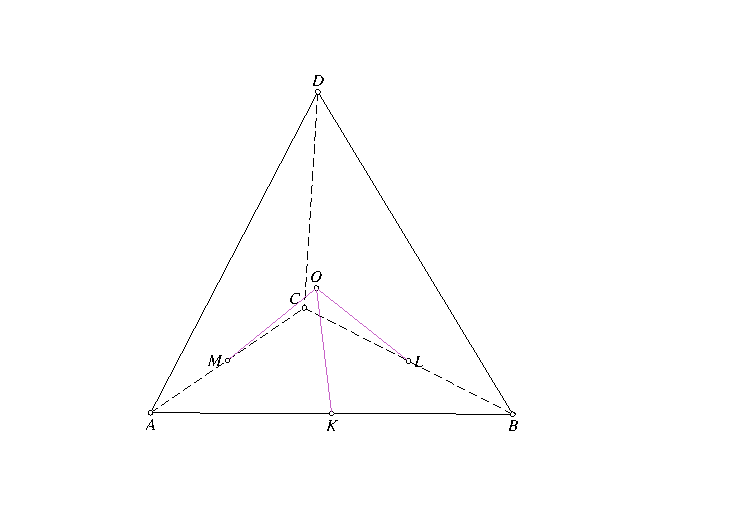
\includegraphics[width=8cm]{./slike/jednaki_uglovi.eps}
  \end{center}
\end{frame}
  
\begin{frame}{Експерименти}
  \begin{center}
    \begin{tabular}{L{1.2cm}||R{1.5cm}|R{1.5cm}|R{1.5cm}|R{1.5cm}|R{0.8cm}}
      \                   &  број полинома & број полинома доказа & просечан број монома & број про\-ме\-нљи\-вих & време \\
      \hline
      \hline
      \textbf{први приступ} & $24$ & $4$ & $7.2$ & $18$ & \emph{Меморијски лимит} \\
      \hline
      \textbf{други приступ} & $24$ & $2$ & $3.5$ & $24$ & $0.835s$
    \end{tabular}
  \end{center}
\end{frame}

\begin{frame}{Експерименти}
  \begin{tabular}{L{1.8cm}||R{1.8cm}|R{1.8cm}|R{1.8cm}|R{1.8cm}}
    \                      & \emph{GeoProver} успех & \emph{GeoProver} неуспех & \emph{Гребнерове базе} успех & \emph{Гребнерове базе} неуспех \\
    \hline
    \hline
    \textbf{први приступ}  &  $13$                  & $16$                     &  $23$                        & $6$  \\
    \hline
    \textbf{други приступ} &  $22$                  & $7$                      &  $29$                        & $0$ \\
  \end{tabular}
\end{frame}

\subsection*{Закључци}

\begin{frame}{Закључци}
  \begin{itemize}
   \item Формализовано је превођење геометријских тврђења у алгебарску
     форму.
   \item Извршена је алгебризација геометријских тврђења на два начина.
   \item Извршено је поређење различитих приступа у алгебризацији.
   \item Тестирањем се показало да је систем ефикаснији када су полиноми
     једноставни.
  \end{itemize}
\end{frame}


%Zakljuci i dalji rad
\section{Даљи рад}

\begin{frame}[shrink]{Даљи рад}
  \begin{itemize}
  \item Доказ да наша дефиниција Декартове координатне равни
    задовољава све аксиоме Хилберта.
  \item Дефинишемо аналитичку геометрију у оквиру аксиоматизације
    Тарског или Хилберта.
  \item Доказати категоричност и система аксиома Тарског и система
    аксиома Хилберта.
  \item Испитати својства различитих класа Мебијусових трансформација.
  \item Завршити формализацију Поинкареовог диск модела.
  \item Испитати примене формализације у другим областима,
    нпр. физици.
  \item Услови недегенерисаности у стереометрији.
  \item Проширити систем тако да обухвати обла тела.
  \item Повезати направљени доказивач са динамичким геометријским
    софтвером.
  \end{itemize}
\end{frame}

\end{document}
